%\section{Accelerated Bayesian Techniques}
% author: Michal Béreš
\label{sec:accelerated_bayes}

% \sts{Standa: Uvod teto sekce je treba najak navazat na predeslou sekci. Doporucil bych zvazit presun teto sekce az na konec seste kapitoly, pripadne do Apendixu na konec zaverecne zpravy.}

This section summarizes practical techniques for accelerating Bayesian inversion in situations where
each evaluation of the forward model $G(u)$ is computationally expensive (e.g.\ PDE-based hydro-mechanical
simulations). The main idea is to reduce the number of expensive model evaluations while preserving
the correct posterior distribution. We focus on \emph{delayed-acceptance Metropolis--Hastings} (DAMH)
sampling (\cite{ChristenFox2005}) combined with adaptive surrogate updates and proposal generation using
short \emph{subchains} (\cite{Subchains}). These methods are implemented in our Python library
\texttt{SurrDAMH} (\cite{surrDAMH}) and are intended as a general toolset for inversion problems of the
type considered throughout this report; the \acrshort{TSX} example below serves only as a benchmark
and a tuning/validation case.

\subsection{Bayesian inverse problem and posterior distribution}
Let $U\in\mathbb{R}^{n}$ denote an unknown parameter vector and let $Y\in\mathbb{R}^{m}$ represent
observations. We assume the additive noise model
\begin{equation}
  Y = G(U) + Z, \qquad Z \sim \mathcal{N}(0, C_Z),
\end{equation}
where $G:\mathbb{R}^{n}\to\mathbb{R}^{m}$ is the observation operator (forward model) and $C_Z$ is
the measurement-noise covariance.

Given observed data $y$, Bayes' formula yields the posterior density (up to a normalizing constant)
\begin{equation}
  \pi(u) := f_{U|Y}(u|y) \propto f_Z\!\bigl(y-G(u)\bigr)\, f_U(u),
\end{equation}
where $f_U$ is the prior density and $f_Z$ is the noise density. For Gaussian noise it is convenient
to use the misfit (negative log-likelihood)
\begin{equation}
  \Phi(u) = \tfrac12 \bigl\|y - G(u)\bigr\|^2_{C_Z^{-1}}
  = \tfrac12 \bigl(y - G(u)\bigr)^\top C_Z^{-1}\bigl(y - G(u)\bigr),
  \label{eq:misfit_phi}
\end{equation}
so that $\pi(u) \propto \exp\!\bigl(-\Phi(u)\bigr)\, f_U(u)$.

\subsection{Metropolis--Hastings sampling}
In most realistic problems the posterior $\pi$ cannot be sampled directly. Metropolis--Hastings (MH)
constructs a \emph{Markov chain} $u^{(0)},u^{(1)},\ldots$ whose stationary distribution is the posterior.
Starting from the current state $u$, MH proposes a candidate $v$ from a proposal distribution
with density $q(\cdot|u)$ and then accepts or rejects $v$ so that, in the long run, the chain spends
time in regions of high posterior probability.

Concretely, the MH acceptance probability is
\begin{equation}
  a(u,v) = \min\!\left(1, \frac{\pi(v)\,q(u|v)}{\pi(u)\,q(v|u)}\right).
  \label{eq:mh_accept}
\end{equation}
A key practical point is that the unknown normalizing constant of $\pi$ cancels in the ratio
$\pi(v)/\pi(u)$, which makes MH usable even when $\pi$ is known only \textquote{up to normalization}.
For symmetric random-walk proposals ($q(v|u)=q(u|v)$), \eqref{eq:mh_accept} simplifies to
$a(u,v)=\min(1,\pi(v)/\pi(u))$.

The computational bottleneck is that evaluating $\pi(v)$ typically requires evaluating $G(v)$,
which can dominate runtime.

\subsection{Delayed-acceptance Metropolis--Hastings (DAMH)}
\label{subsec:damh}
Delayed acceptance (\cite{ChristenFox2005}) introduces a cheap approximation of the posterior, constructed
from a surrogate $\widetilde{G}(u)\approx G(u)$:
\begin{equation}
  \widetilde{\pi}(u) \propto f_Z\!\bigl(y-\widetilde{G}(u)\bigr)\, f_U(u).
\end{equation}
Each proposal is tested first using the surrogate; only proposals that pass the first test require an
expensive evaluation of the full model.

Figure~\ref{fig:damh_two_stage} illustrates this two-stage logic. The important property is that the
resulting Markov chain still targets the \emph{exact} posterior $\pi$ (the second stage corrects the
approximation error).

\begin{figure}[t]
  \centering
  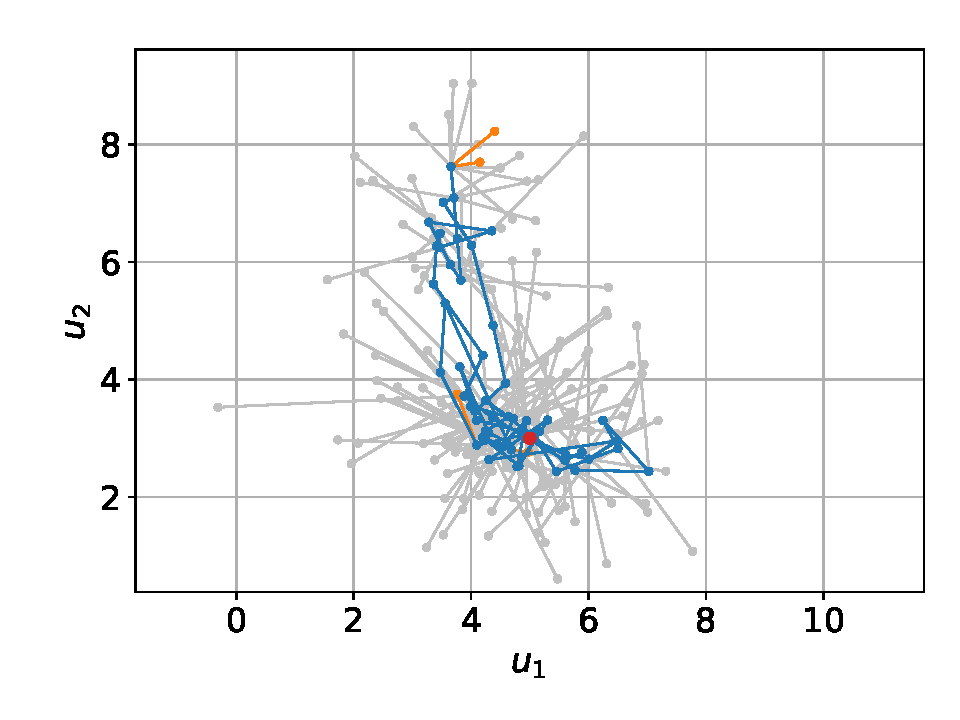
\includegraphics[width=0.6\linewidth]{fig_bayes/damh_two_stage}
  \caption{Two-stage delayed acceptance.}
  \label{fig:damh_two_stage}
\end{figure}

\subsubsection{Two-stage acceptance rule}
Given current state $u$, DAMH proceeds as follows:
\begin{mdframed}
\noindent\textbf{DAMH (two-stage acceptance).}
\begin{enumerate}
\item Propose $v \sim q(\cdot|u)$.
\item \textbf{Stage 1 (surrogate screening):} pre-accept with probability
\[
\widetilde{a}(u,v)=\min\!\left(1,\frac{\widetilde{\pi}(v)\,q(u|v)}{\widetilde{\pi}(u)\,q(v|u)}\right).
\]
If rejected, set the next sample to $u$.
\item \textbf{Stage 2 (exact correction):} if Stage 1 is passed, evaluate $G(v)$ and accept with probability
\[
a_2(u,v)=\min\!\left(1,\frac{\pi(v)\,\widetilde{\pi}(u)}{\pi(u)\,\widetilde{\pi}(v)}\right).
\]
\end{enumerate}
\end{mdframed}

\subsubsection{Adaptive surrogate updates (DAMH-SMU)}
In practice, a fixed surrogate is rarely sufficient. DAMH-SMU updates the surrogate during sampling,
using a growing set of \emph{snapshots}
\begin{equation}
  \mathcal{S}=\bigl\{(u^{(i)},\, G(u^{(i)}))\bigr\}_{i=1}^{N_S}.
\end{equation}
At iteration $k$, a surrogate $\widetilde{G}^{(k)}$ is trained (or refined) on $\mathcal{S}$, yielding
$\widetilde{\pi}^{(k)}$. After proposing $v$ and performing the exact correction, the pair $(v,G(v))$
is appended to $\mathcal{S}$. This adaptive process typically decreases the amount of wasted full-model
evaluations as the surrogate improves.

\subsubsection{Proposal subchains on the surrogate posterior}
\label{subsec:subchains}
To improve mixing (reduce correlation between successive samples), proposals can be generated by a short
MH \emph{subchain} that targets the surrogate posterior $\widetilde{\pi}^{(k)}$ (\cite{Subchains}). Starting
from the current state $u^{(k)}$, we run $m_{\max}$ surrogate-only MH steps to obtain a proposal $v$,
which is then corrected using one full evaluation of $G$.

\begin{mdframed}
\noindent\textbf{DAMH-SMU with proposal subchains.} For $k=0,1,\dots$:
\begin{enumerate}
\item Build/update $\widetilde{G}^{(k)}$ from snapshots $\mathcal{S}$ and define $\widetilde{\pi}^{(k)}$.
\item Set $w^{(0)} = u^{(k)}$. For $m=0,\dots,m_{\max}-1$:
\begin{enumerate}
\item Propose $z\sim q^{(k)}(\cdot|w^{(m)})$.
\item Accept $z$ as $w^{(m+1)}$ with probability
\[
\widetilde{a}\bigl(w^{(m)},z\bigr)=\min\!\left(1,\frac{\widetilde{\pi}^{(k)}(z)\,q^{(k)}(w^{(m)}|z)}
{\widetilde{\pi}^{(k)}(w^{(m)})\,q^{(k)}(z|w^{(m)})}\right).
\]
\end{enumerate}
\item Set proposal $v = w^{(m_{\max})}$.
\item Perform the exact correction using the full model:
\[
a_2\bigl(u^{(k)},v\bigr)=\min\!\left(1,\frac{\pi(v)\,\widetilde{\pi}^{(k)}(u^{(k)})}
{\pi(u^{(k)})\,\widetilde{\pi}^{(k)}(v)}\right).
\]
\item Append $(v,G(v))$ to $\mathcal{S}$ if $G(v)$ was evaluated.
\end{enumerate}
\end{mdframed}

\subsubsection{Surrogate models used in this work (overview)}
The \texttt{SurrDAMH} framework (see \cite{surrDAMH}) supports several non-intrusive surrogates $\widetilde{G}$
trained from the snapshot set $\mathcal{S}$. In the benchmark considered below we used a neural network
surrogate: a multilayer perceptron (MLP) trained on normalized inputs/outputs (approximately
$\mathcal{N}(0,1)$). The surrogate is updated online as new snapshots become available.

\subsection{Benchmark application: TSX heterogeneous poroelastic model}
\label{subsec:tsx_subdomains}
In order to validate and tune the sampling and surrogate-update strategy, we use a benchmark motivated
by the \acrshort{TSX} experiment (\cite{rutqvist2009modeling}). The benchmark is representative of the class of inverse
problems relevant for this report: a coupled poroelastic forward model, multiple uncertain parameters,
and time-dependent pore-pressure observations. The same workflows (construction of $\pi(u)$ from
\eqref{eq:misfit_phi}, MH/DAMH sampling, and surrogate acceleration) are directly transferable to other
pore-pressure inversion tasks.

\subsubsection{Forward model and observed data}
We consider quasi-static Biot poroelasticity:
\begin{align}
  -\div\!\bigl(\mathbb{C}:\varepsilon(\uu)\bigr) + \alpha_{B}\nabla p &= 0, \\
  c_{pp}\,\prtl_t p - \nabla\cdot\!\left(\frac{k}{\mu}\nabla p\right)
  + \alpha_{B}\,\prtl_t\bigl(\div(\uu)\bigr) &= 0,
\end{align}
where $\uu$ is displacement, $p$ is pore pressure, $k/\mu$ is hydraulic conductivity, $c_{pp}$ is
storativity, and $\alpha_B$ is the Biot--Willis coefficient. We assume isotropic linear elasticity
\begin{equation}
  \mathbb{C}:\varepsilon(\uu) = 2G\,\varepsilon(\uu) + \lambda\,(\div \uu)\,I,
  \qquad
  \lambda = \frac{E\nu}{(1+\nu)(1-2\nu)}, \quad G=\frac{E}{2(1+\nu)}.
\end{equation}

The observed dataset consists of four pore-pressure time series measured at four control points over
approximately one year. The control-point locations are shown in Fig.~\ref{fig:tsx_tunnel_points}.
For orientation, the subdomain partition used in the heterogeneous model is shown in
Fig.~\ref{fig:tsx_geometry}.

\begin{figure}[t]
  \centering
  \begin{subfigure}[t]{0.49\linewidth}
    \centering
    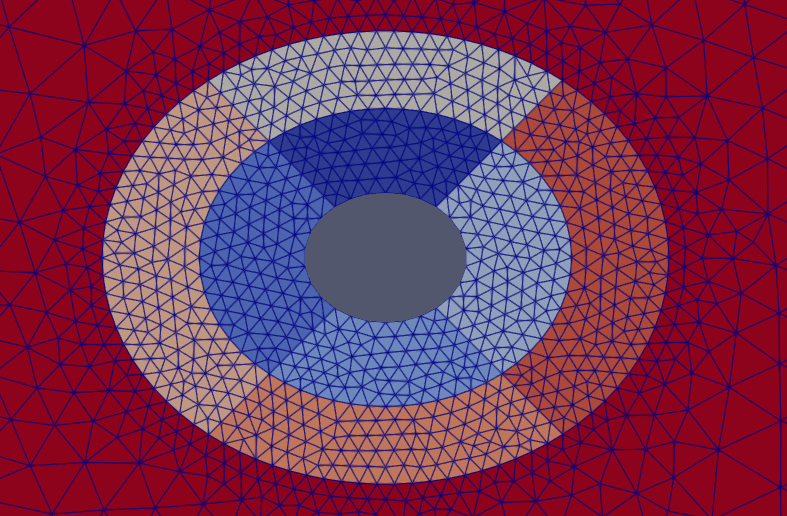
\includegraphics[height=0.6\linewidth]{fig_bayes/Paraview_detail.png}
    \caption{Subdomain layout.}
    \label{fig:tsx_geometry}
  \end{subfigure}
  \hfill
  \begin{subfigure}[t]{0.49\linewidth}
    \centering
    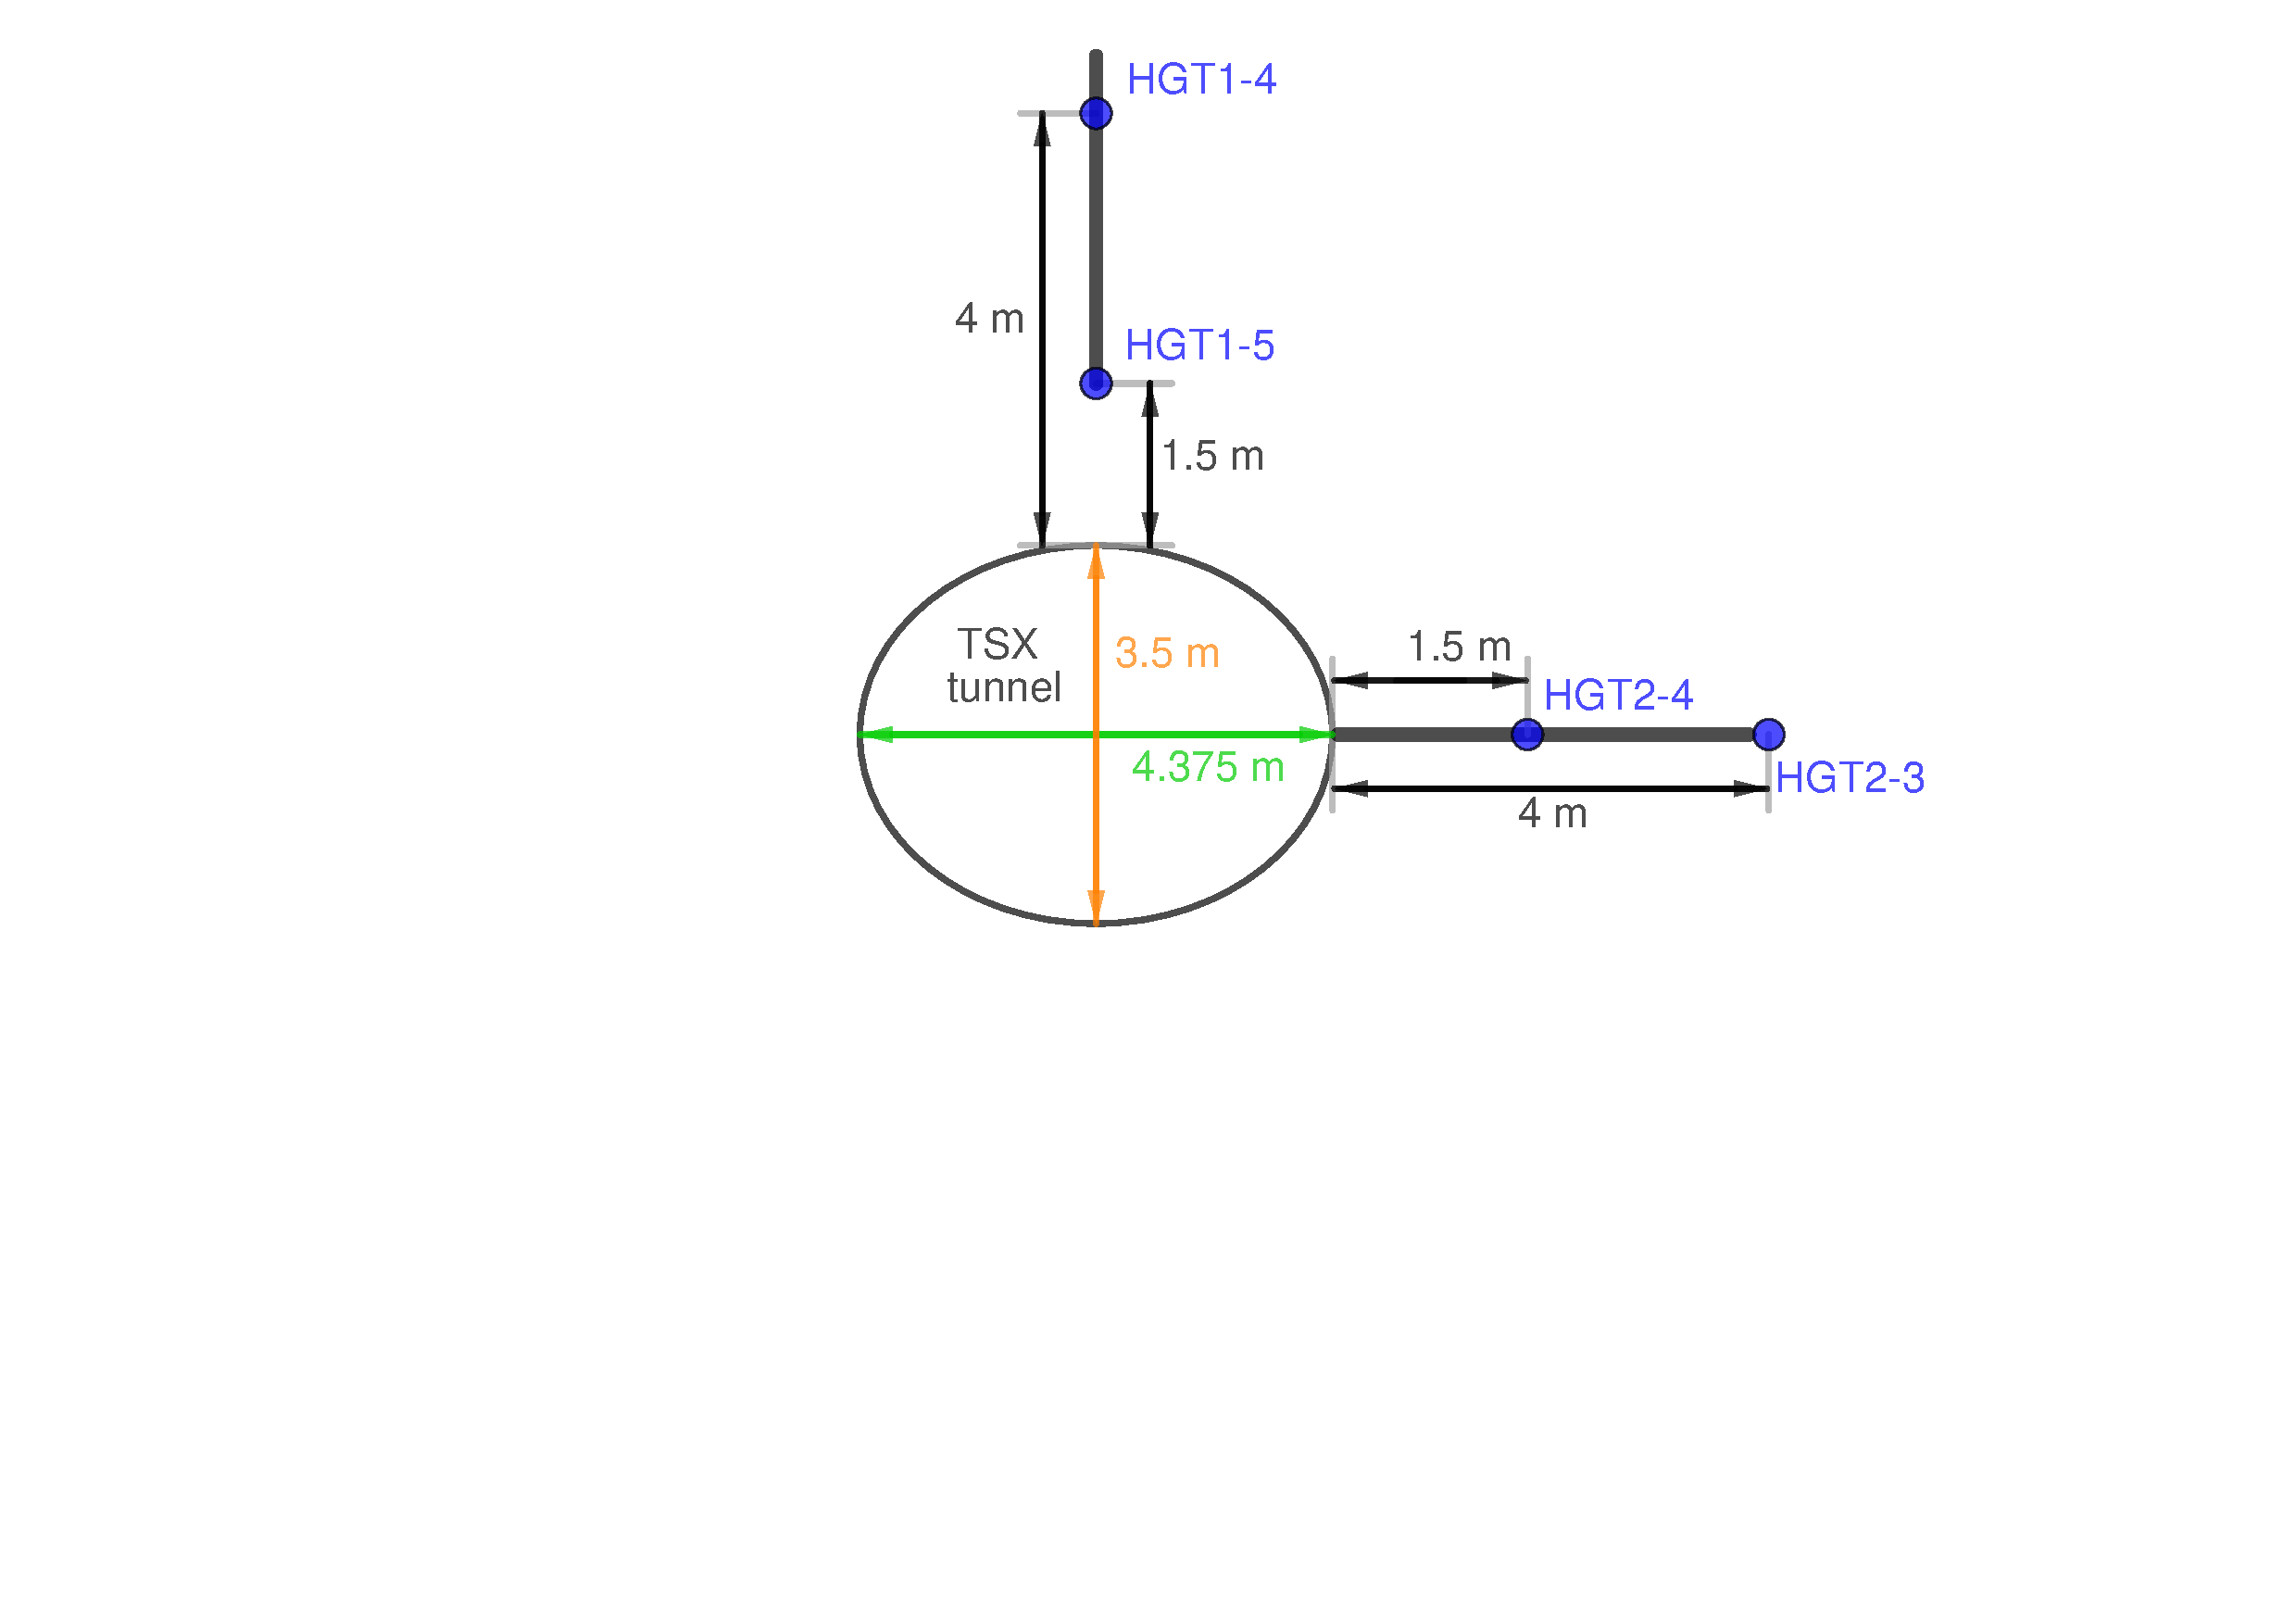
\includegraphics[height=0.6\linewidth]{fig_bayes/TSX_tunnel_flipped_2.pdf}
    \caption{Tunnel cross-section and control points.}
    \label{fig:tsx_tunnel_points}
  \end{subfigure}
  \caption{Geometry used in the TSX benchmark.}
  \label{fig:tsx_setting}
\end{figure}

Figure~\ref{fig:tsx_best_fit} visualizes the measurements together with a best-fitting model output
$G(u_{\mathrm{best}})$ among the generated samples. This figure is used mainly to confirm that the
heterogeneous model is able to match all four time series simultaneously.

\begin{figure}[t]
  \centering
  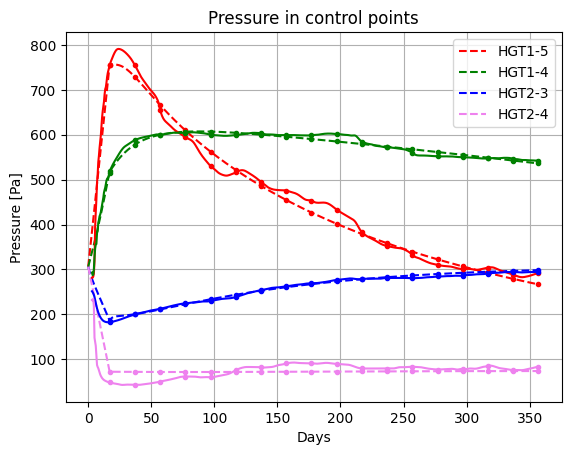
\includegraphics[width=0.68\linewidth]{fig_bayes/tsx_best_fit_timeseries}
  \caption{Measured time series and best-fit simulator output.}
  \label{fig:tsx_best_fit}
\end{figure}

\subsubsection{Unknown parameters and dimension}
The benchmark uses a piecewise-homogeneous parametrization on $N_{\mathrm{sub}}=9$ subdomains (two rings
with four subdomains each, plus an outer region). In each subdomain we estimate constant values of
\[
\frac{k}{\mu}, \quad c_{pp}, \quad E, \quad \nu,
\]
which yields $4\times 9 = 36$ material parameters. In addition, the initial stress tensor is parametrized
by principal stress magnitudes $\sigma_x,\sigma_y$ and orientation angle $\alpha$. Altogether,
\[
n = 36 + 3 = 39,
\qquad
G:\mathbb{R}^{39}\to\mathbb{R}^{144}
\]
for the dataset considered.

\subsubsection{Example posterior summaries (permeability)}
As a representative example of spatially resolved results, Fig.~\ref{fig:tsx_perm_results} shows the
posterior mean and posterior standard deviation of permeability in terms of $\log_{10}(k/\mu)$.
Subdomains that contain (or are close to) control points typically become well-informed by the data,
while others remain closer to the prior with high posterior variance.

\begin{figure}[t]
  \centering
  \begin{subfigure}[t]{0.49\linewidth}
    \centering
    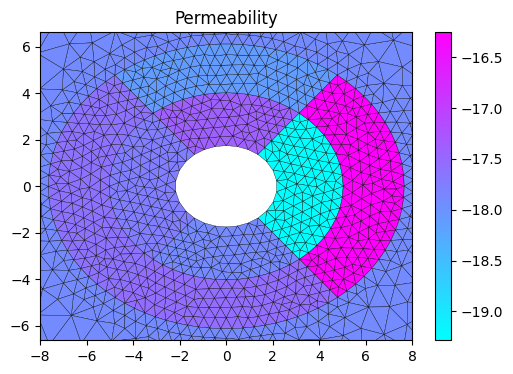
\includegraphics[
      height=0.6\linewidth,
      trim=0 0 0 21,
      clip
    ]{fig_bayes/mean_permeability}
    \caption{Posterior mean.}
    \label{fig:tsx_perm_mean}
  \end{subfigure}
  \hfill
  \begin{subfigure}[t]{0.49\linewidth}
    \centering
    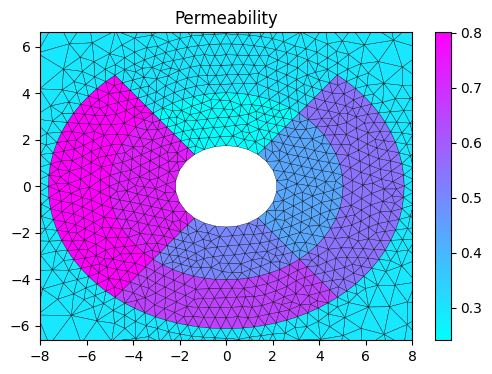
\includegraphics[
      height=0.6\linewidth,
      trim=0 0 0 21,
      clip
    ]{fig_bayes/std_permeability}
    \caption{Posterior standard deviation.}
    \label{fig:tsx_perm_std}
  \end{subfigure}
  \caption{Posterior summaries for $\log_{10}(k/\mu)$.}
  \label{fig:tsx_perm_results}
\end{figure}


\subsection{Sampling efficiency measure: travelled distance in normalized space}
\label{subsec:efficiency_distance}
Classical MCMC efficiency measures (integrated autocorrelation time, effective sample size) are useful,
but in practice they can be noisy unless chains are very long. For runtime monitoring we therefore use a
simple, robust proxy: the \emph{Euclidean distance travelled} by the chain in normalized parameter space.

Let $\hat{u}^{(0)},\ldots,\hat{u}^{(N)}$ be the MCMC samples after normalization, where each parameter
component is scaled so that the prior is approximately $\mathcal{N}(0,1)$. We define
\begin{equation}
  d \;=\; \sum_{i=1}^{N} \left\lVert \hat{u}^{(i)} - \hat{u}^{(i-1)} \right\rVert_{2}.
  \label{eq:chain_distance}
\end{equation}
Larger $d$ indicates better exploration per unit computational effort (fewer repeated states, better mixing).

Figure~\ref{fig:sampling_quality} reports this distance over a long TSX run. The run is divided into fixed
time segments; within each segment, multiple chains are generated in parallel and share a single surrogate model.
As surrogate refinements accumulate, we can allow longer subchains without risking costly model rejections. Consequently, the
travelled distance increases. The same plot also provides a reference run using an optimally tuned pure MH algorithm. The theoretically
maximal limit of a chain length (i.e., an upper bound) for an \emph{ideal} sampling procedure (a perfect surrogate with infinite subchain
length and no computational cost); the \textquote{Monte Carlo ceiling} corresponding to independent sampling under the same runtime budget; would yield a travel distance of around 3700 (simulated value).


\begin{figure}[t]
  \centering
  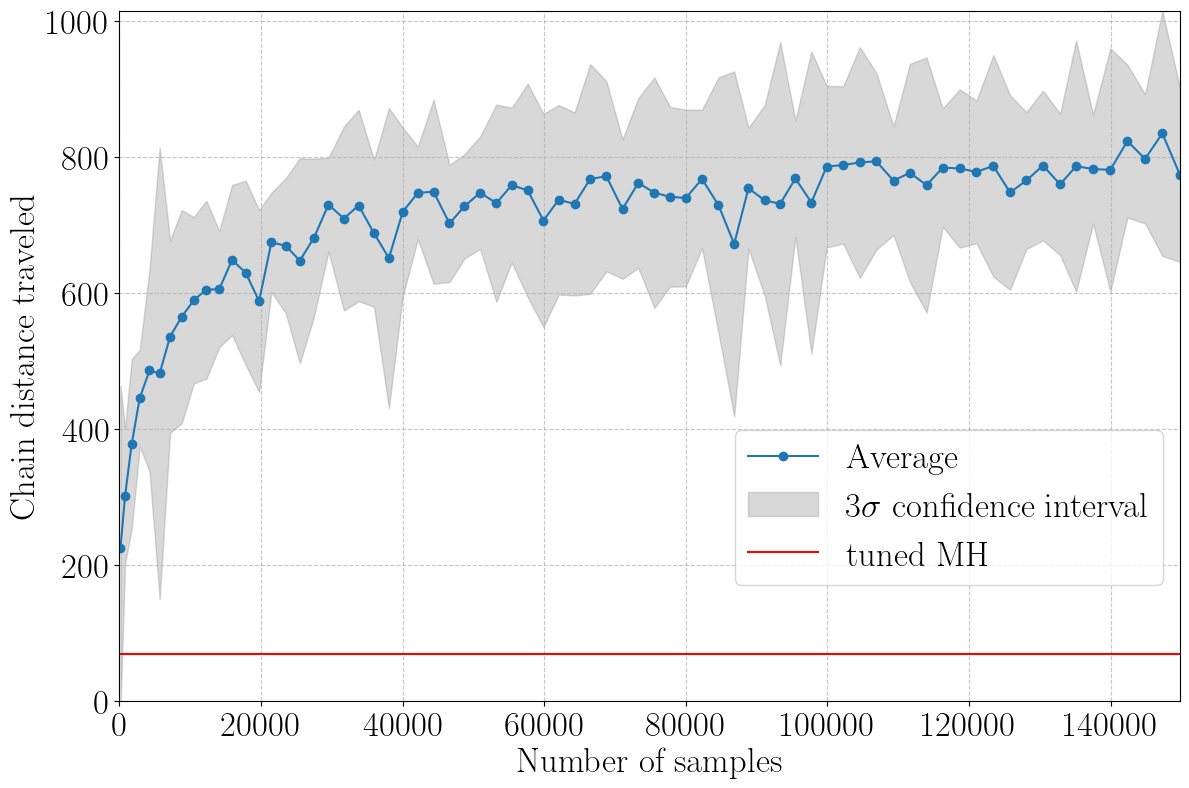
\includegraphics[width=0.70\linewidth]{fig_bayes/samling_quality}
  \caption{Travelled distance proxy for sampling efficiency.}
  \label{fig:sampling_quality}
\end{figure}

\subsection{Software implementation (\texttt{SurrDAMH})}
The algorithms above are implemented in \texttt{SurrDAMH} (\cite{surrDAMH}), a general-purpose library for MH,
DAMH, and DAMH-SMU sampling with optional surrogate subchains and adaptive proposal mechanisms
(e.g.\ Adaptive Metropolis (\cite{Haario})). The library is designed for expensive forward models: it supports
MPI-based parallelism in which multiple sampler processes generate chains while sharing (i) a single surrogate
updated by a dedicated process and (ii) a pool of forward-model solvers for full evaluations of $G$.

Figure~\ref{fig:surrdamh_parallel} sketches the parallel structure. The key practical advantage is that the
number of solver processes can be smaller than the number of Markov chains, keeping the expensive solvers busy
while sampler processes continue with cheap surrogate work.

\begin{figure}[t]
  \centering
  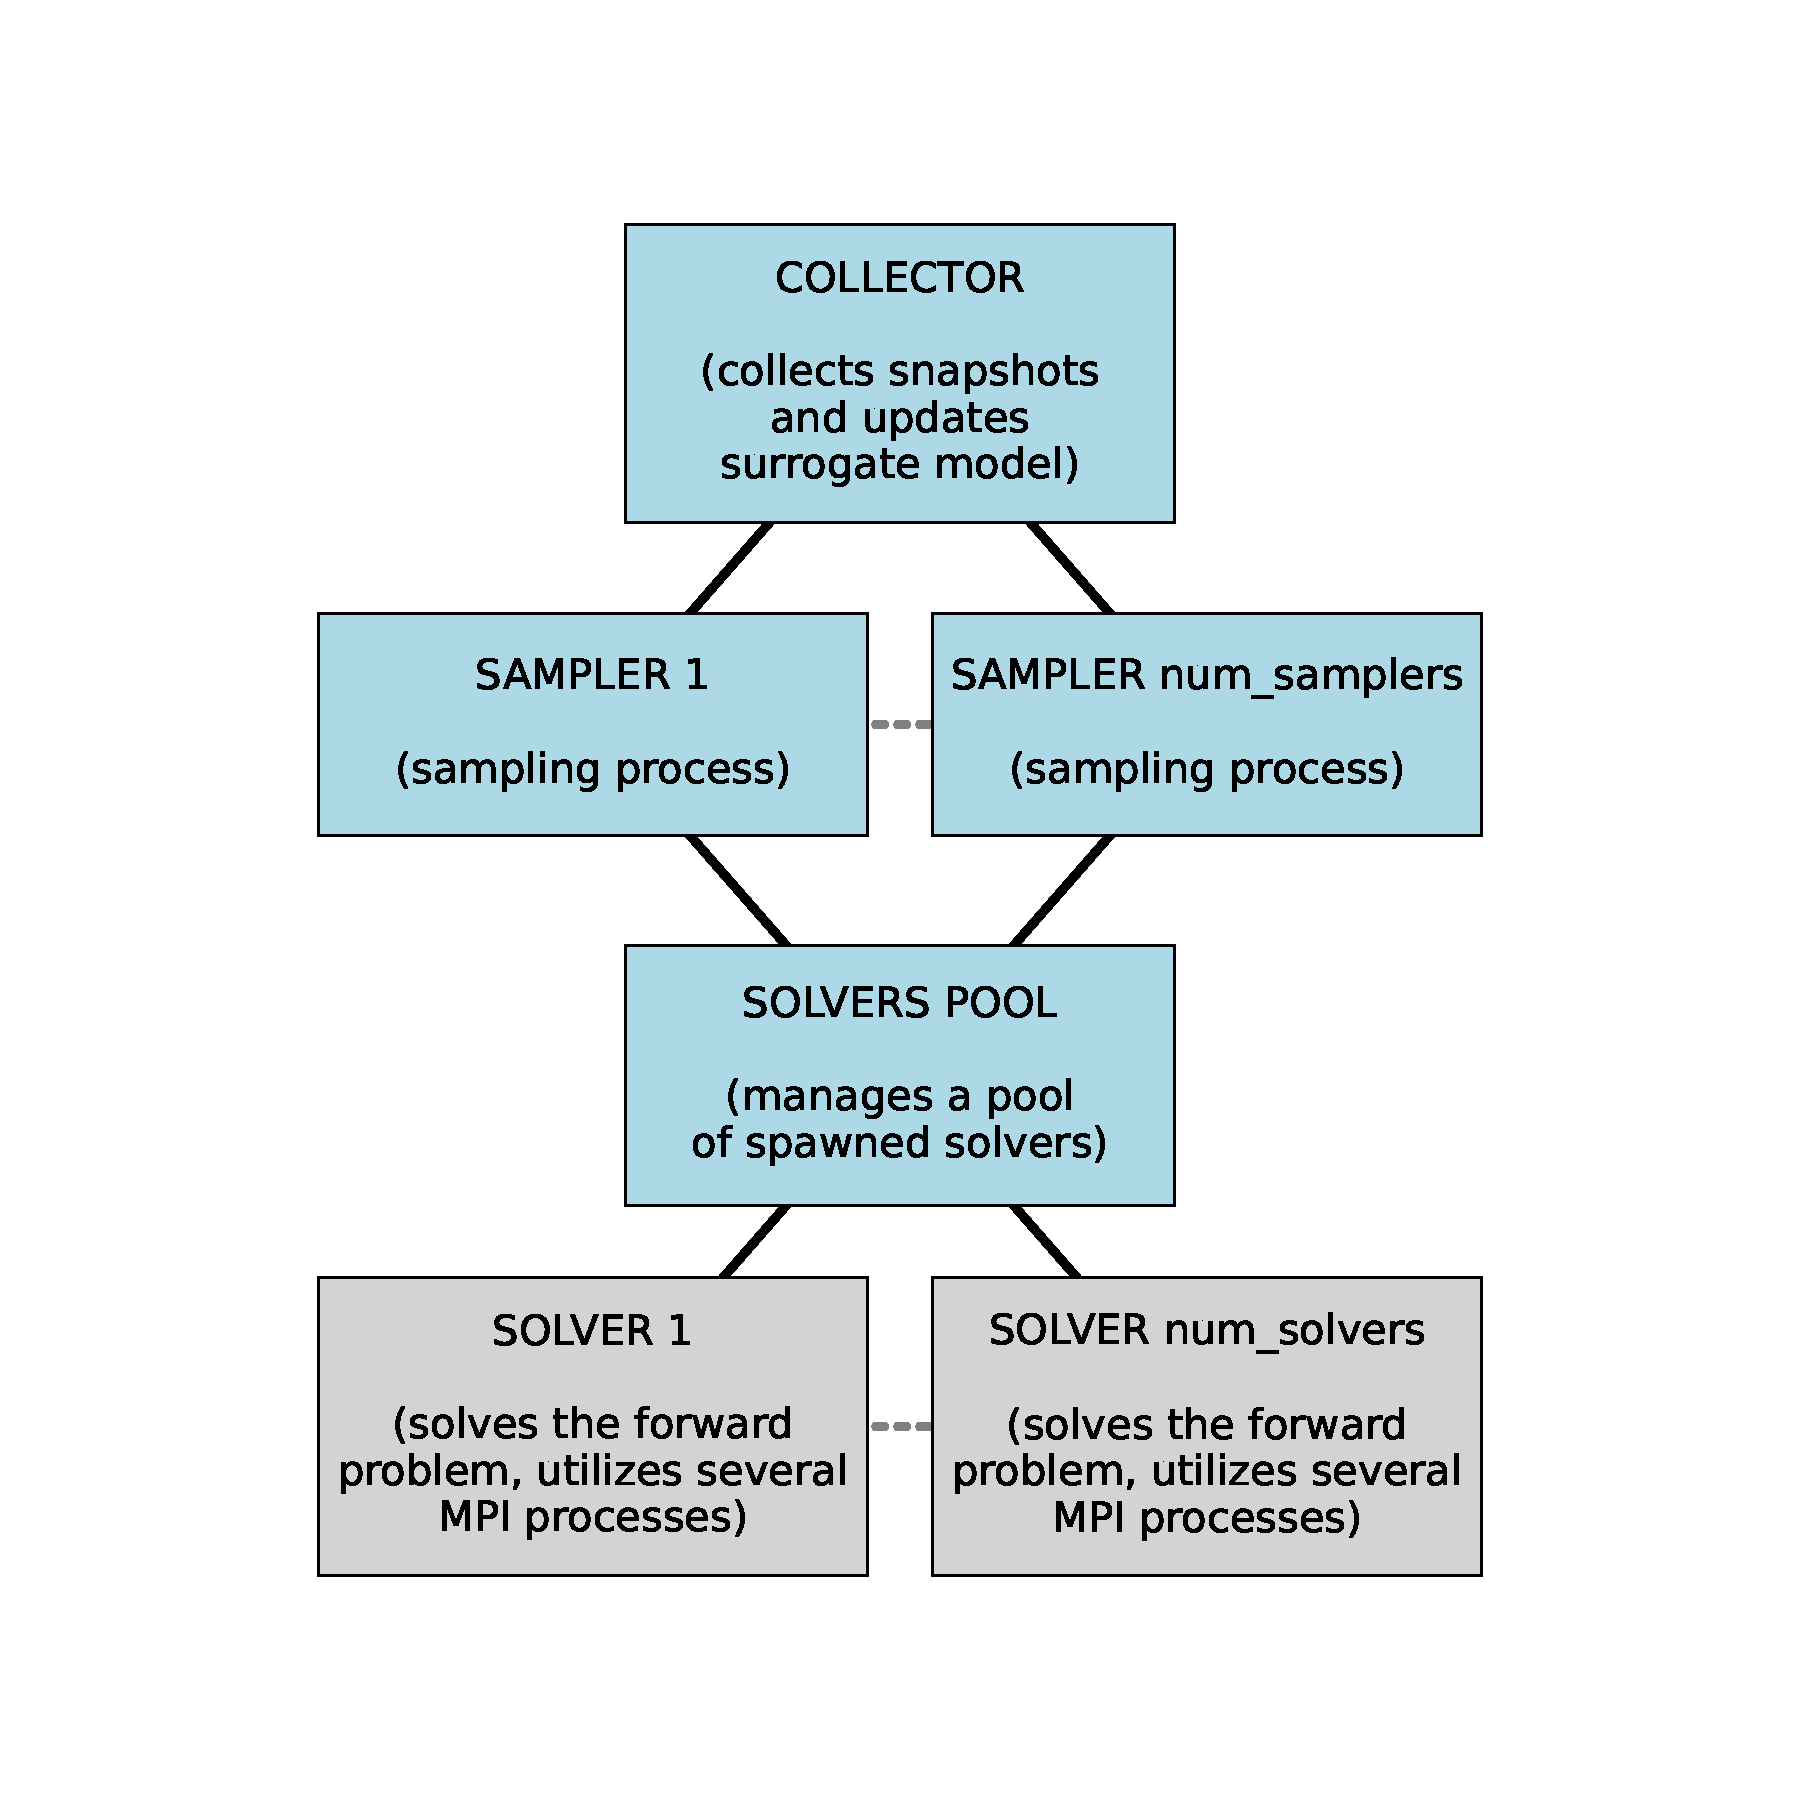
\includegraphics[width=0.82\linewidth]{fig_bayes/surrdamh_parallel_scheme}
  \caption{Parallel layout of \texttt{SurrDAMH}.}
  \label{fig:surrdamh_parallel}
\end{figure}

\subsection{Summary}
Delayed acceptance (\cite{ChristenFox2005}), adaptive surrogate refinement, and surrogate-subchain proposals
(\cite{Subchains}) provide a practical route to Bayesian inversion in computationally demanding settings.
We have applied these techniques on the TSX benchmark inversion problem (\cite{rutqvist2009modeling}), demonstrating identification of significant heterogeneity in the hydraulic and elastic properties of the rock mass.  This approach, as implemented in the \texttt{SurrDAMH} library (\cite{surrDAMH}), enables systematic inference of rock mass heterogeneity from the Pore Pressure experiment.
